\documentclass[letterpaper]{article}

\usepackage{Bioconductor}
\usepackage{graphicx}
\usepackage{fullpage}
\title{\Bioconductor{} Annual Report for 2021}
\author{Lori Kern\\ Roswell Park Comprehensive Cancer Center \\ Vincent Carey \\ Harvard Medical School}
\date{Oct 13, 2022; production delayed}

\begin{document}

\maketitle

\tableofcontents

\pagebreak

\section{Project Scope}

\Bioconductor{} provides access to software for the analysis and
comprehension of high throughput genomic data. Packages are written in
the \R{} programming language by members of the \Bioconductor{} team
and the international community. \Bioconductor{} was started in Fall,
2001 by Dr.\ Robert Gentleman and others, and now consists of 2083
software packages for the analysis of data ranging from single-cell
sequencing to flow cytometry.

The mission of the Bioconductor project is to develop, support, and disseminate
free open source software that facilitates rigorous and reproducible analysis of
data from current and emerging biological assays. We are dedicated to building a
diverse, collaborative, and welcoming community of developers and data
scientists.

\subsection{Funding}

A summary of projects funded for domestic investigators and 
collaborators is given in Table \ref{gra}.

% latex table generated in R 4.2.1 by xtable 1.8-4 package
% Thu Oct 13 19:44:41 2022
\begin{table}[ht]
\centering
\begin{tabular}{rlllll}
  \hline
 Institute-Topic-Type & Project Number & PIs & Start & End \\ 
  \hline
 NHGRI Bioconductor U24 & 2U24HG004059-17 & Irizarry;Carey & 3/2021 & 3/2026 \\ 
 NHGRI AnVIL U24 & 5U24HG010263-05 & Schatz/MPIs & 9/2018 & 7/2023 \\ 
 NCI ITCR U24 & 5U24CA180996-08 & Waldron;Morgan & 9/2019 & 9/2024  \\ 
 NCI Metagenomics U01 & 1U01CA230551-01A1 & Waldron & 7/2020 & 7/2024 \\ 
 NIH Common Fund R03 & 1R03OD032629-01 & Carey;Culhane & 9/2021 & 9/2023 \\ 
 NSF ACCESS cloud & BIR190004 & Carey & 3/2022 & 3/2023 \\ 
   \hline
\end{tabular}
\caption{Summary of grants to domestic investigators.}
\label{gra}
\end{table}

Figure \ref{fig:org-chart} provides an approximate view of
relationships among investigators and staff and their tasks.
Institutions are Dana-Farber Cancer Institute (DFCI),
Brigham and Women's Hospital (BWH), RPCI (Roswell Park
Cancer Institute), City University of New York (CUNY), and
Fred Hutchinson Cancer Research Center (FHCRC).  Abbreviations
in use include CAB (Community Advisory Board), TAB (Technical
Advisory Board), PM (Project Management), BBS (Bioconductor 
Build System), AnVIL (Analysis and Visualization Lab Space, and
NHGRI Cloud Computing initiative.)  "Hubs" refers to AnnotationHub
and ExperimentHub resources provided by the project.  "BSgenome/Forges"
refers to a collection of systems for representing reference genomes
using Biostrings.

%name	institute	task	super
%R. Irizarry	DFCI	PI/methods	Bioc
%V. Carey	BWH	PI/tech/TAB	Bioc
%N. George	DFCI	Hardware	R. Irizarry
%N. Breslin	DFCI	Grants	R. Irizarry
%sub1	BWH	Carey/Mahmoud	N. Breslin
%sub2	RPCI	Morgan/Kern/Interdonato	N. Breslin
%sub3	CUNY	Waldron/Wokaty/Ramos	N. Breslin
%sub4	FHCRC	BSgenome/Forges	N. Breslin
%K. Street	DFCI	methods	R. Irizarry
%%(TBN)	DFCI	CoreDev	V. Carey
%L. Kern	RPCI	PM/Hubs/CAB	V. Carey
%H. Pages	FHCRC	BBS/stack	V. Carey
%J. Wokaty	CUNY	BBS/outreach	H. Pages
%A. Mahmoud	BWH	Cloud/AnVIL	V. Carey
%A. Culhane	Limerick	methods/CZI/DI	Bioc
%M. Doyle	Limerick	Comm. Mgr.	A. Culhane
%K. Interdonato	RPCI	Hubs/Anno	L. Kern

\begin{figure}[b]
  \begin{center}
    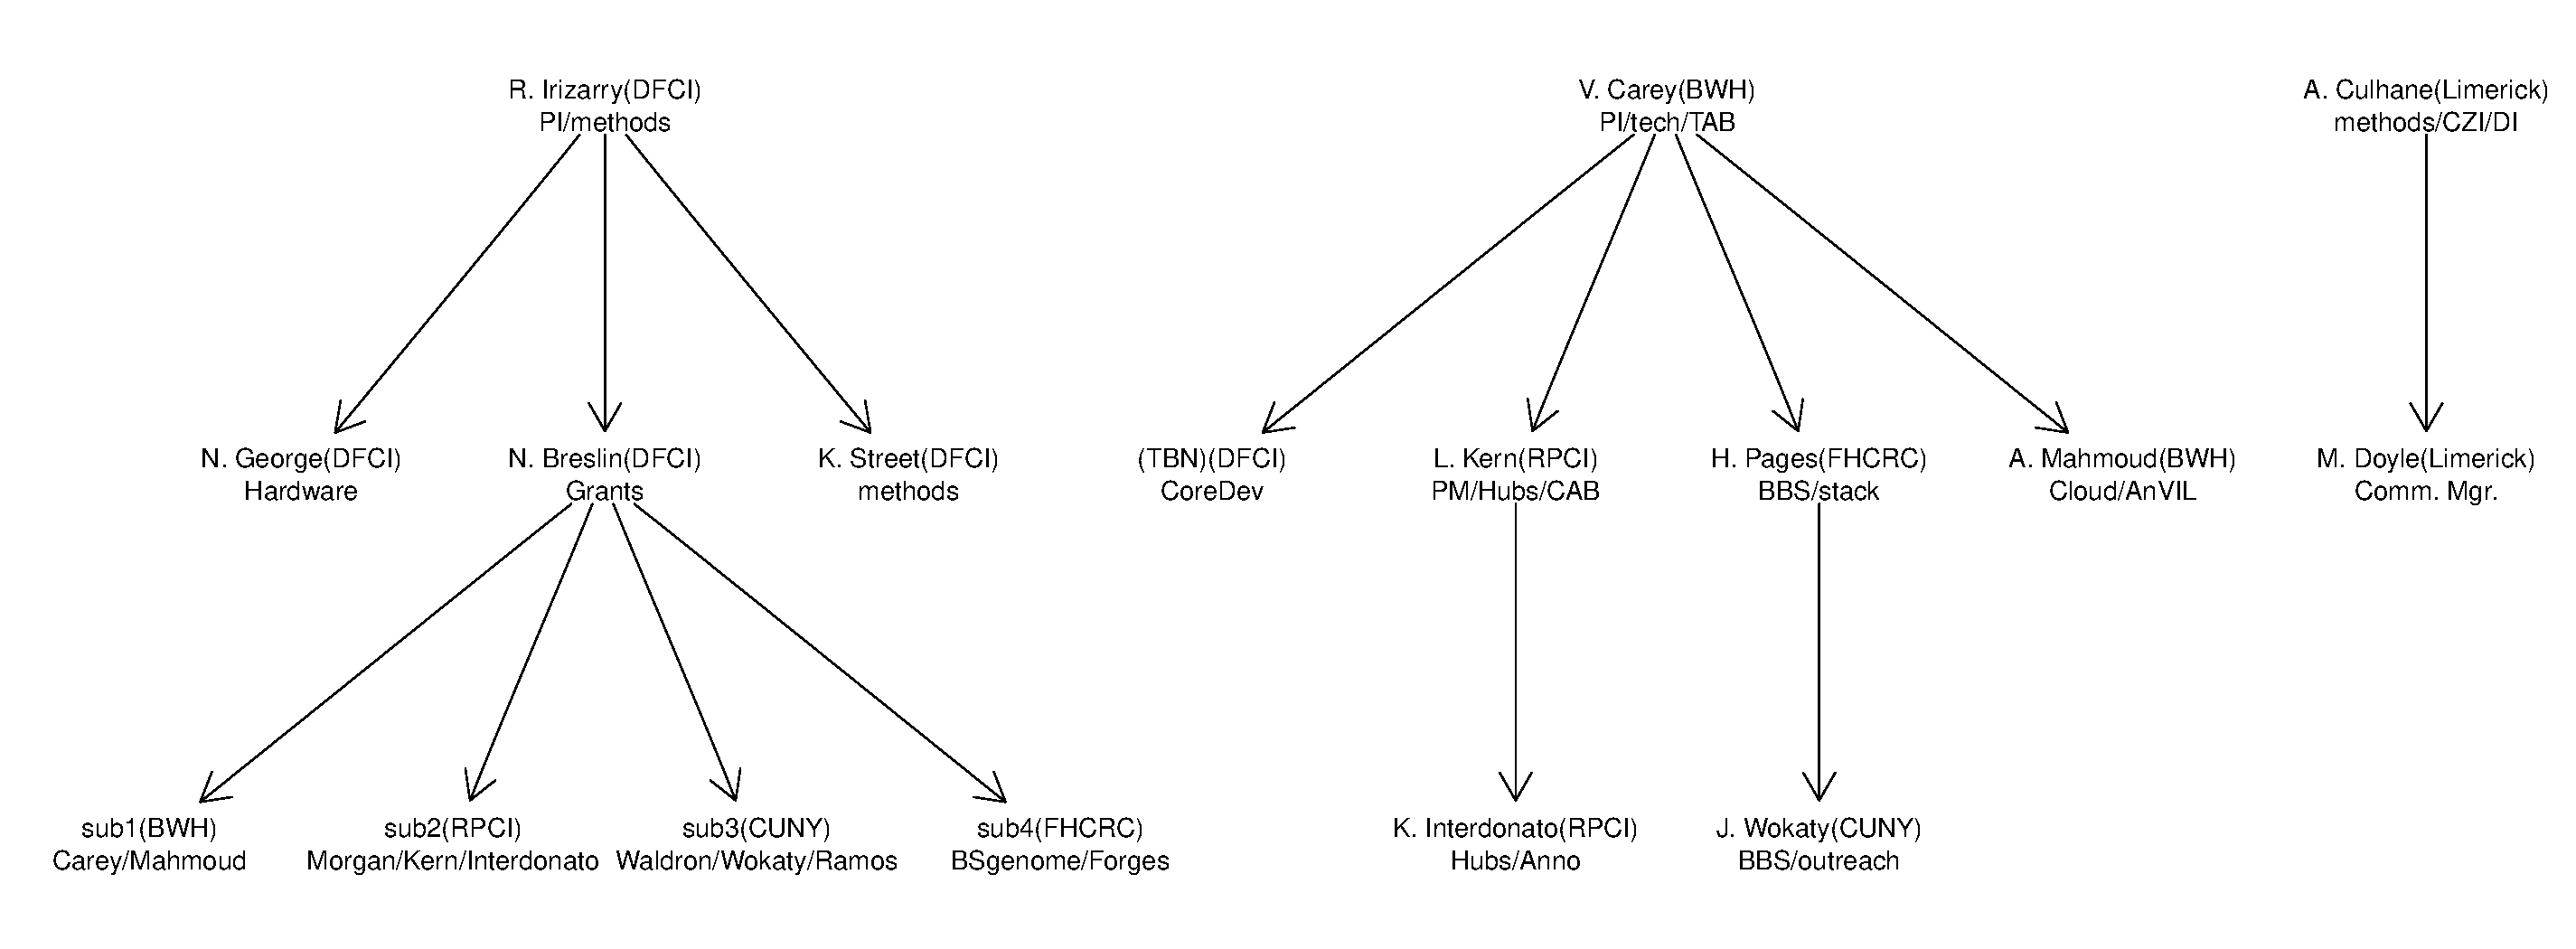
\includegraphics[width=1.1\textwidth,height=!]{newgr2}
    \caption{Organizational chart.}
    \label{fig:org-chart}
  \end{center}
\end{figure}



\subsection{Package and Annotation Resources}

\R{} software packages represent a primary product of the
\Bioconductor{} project. Packages are produced by the \Bioconductor{}
team and from international
contributors.  There are several types of package to be distinguished.

\begin{itemize}
\item \textbf{Central infrastructure}.  This includes packages that
provide formal programming support.
Exampls include
BiocGenerics,
S4Vectors,
BiocVersion,
IRanges,
Biobase,
zlibbioc,
XVector,
BiocParallel,
DelayedArray,
MatrixGenerics, graph, rhdf5.
\item \textbf{Genome representation support}.  This includes
Biostrings, BSgenome, GenomeInfoDb, GenomicRanges.
\item \textbf{Infrastructure for high-throughput sequencing data.}
Includes Rsamtools, Rhtslib, tximport, GenomicAlignments, Rsubread, Rbowtie.
\item \textbf{Experiment representation support}.  Examples are
SummarizedExperiment, SingleCellExperiment, SpatialExperiment.
\item \textbf{Annotation support}.
org.Hs.eg.db, GO.db, TxDb.Hsapiens.UCSC.hg38.knownGene
\item \textbf{Analysis of genome-scale data}.  Most of the 2000+
packages curated by the project address details of genome-scale
analysis.  Highly ranked (by recorded number of downloads)  
analysis packages include limma, edgeR, DESeq2, clusterProfiler, VariantAnnotation, sva.
\end{itemize}

Table~\ref{tbl:analysis_pkgs} summarizes growth in the
number of packages hosted by \Bioconductor{}, with
\href{https://bioconductor.org/packages/3.14}{2083 software packages}
available in release 3.14.  The project produces 901 `annotation'
packages to help researchers place analytic results into biological
context. Annotation packages are curated resources derived from
external data sources, and are updated at each release. The project
also produces 408 `experiment data' packages to provide heavily
curated results for pedagogic and comparative purposes. We have
standardized reproducible, cross-package protocols into 29 `workflow'
packages. There are also
\href{http://bioconductor.org/checkResults/3.14/books-LATEST/}{8 `books`} for
in-depth analysis mostly focused on Single Cell Analysis.


The project has developed, over the last several years, the
`AnnotationHub' and `ExperimentHub` resources for serving and managing
genome-scale annotation data, e.g., from the TCGA, NCBI, and
Ensembl. There are 60134 records in the AnnotationHub, and 6075
ExperimentHub records.

The number of distinct IP addresses downloading software continues to
grow in an approximately exponential fashion
(Figure~\ref{fig:download-stats}).

\begin{table}[b]
  \begin{center}
    \caption{Number of contributed packages included in each
      \Bioconductor{} release.  Releases occur twice per year.}
    \label{tbl:analysis_pkgs}
    \begin{tabular}{llc|llc|llc|llc|llc}
      \\
      \multicolumn{2}{l}{Release} & N & 
      \multicolumn{2}{l}{Release} & N & 
      \multicolumn{2}{l}{Release} & N &
      \multicolumn{2}{l}{Release} & N \\\hline\noalign{\smallskip}
      2002 & 1.0 & 15    & 2006 & 1.8 & 172  & 2010 & 2.6 & 389 & 2014 & 2.14 & 824  & 2018 & 3.7  & 1560\\ 
           & 1.1 & 20    &      & 1.9 & 188  &      & 2.7 & 419 &      & 3.0  & 936  &      & 3.8  & 1649\\
      2003 & 1.2 & 30    & 2007 & 2.0 & 214  & 2011 & 2.8 & 467 & 2015 & 3.1  & 1024 & 2019 & 3.9  & 1741\\
           & 1.3 & 49    &      & 2.1 & 233  &      & 2.9 & 517 &      & 3.2  & 1104 &      & 3.10 & 1823\\
      2004 & 1.4 & 81    & 2008 & 2.2 & 260  & 2012 & 2.10 & 554& 2016 & 3.3  & 1211 & 2020 & 3.11 & 1903\\
           & 1.5 & 100   &      & 2.3 & 294  &      & 2.11 & 610&      & 3.4  & 1294 &      & 3.12 & 1974\\
      2005 & 1.6 & 123   & 2009 & 2.4 & 320  & 2013 & 2.12 & 671& 2017 & 3.5  & 1381 & 2021 & 3.13 & 2042\\
           & 1.7 & 141   &      & 2.5 & 352  &      & 2.13 & 749&      & 3.6  & 1473 &      & 3.14 & 2083\\
    \end{tabular}
  \end{center}
\end{table}

\begin{figure}
  \begin{center}
    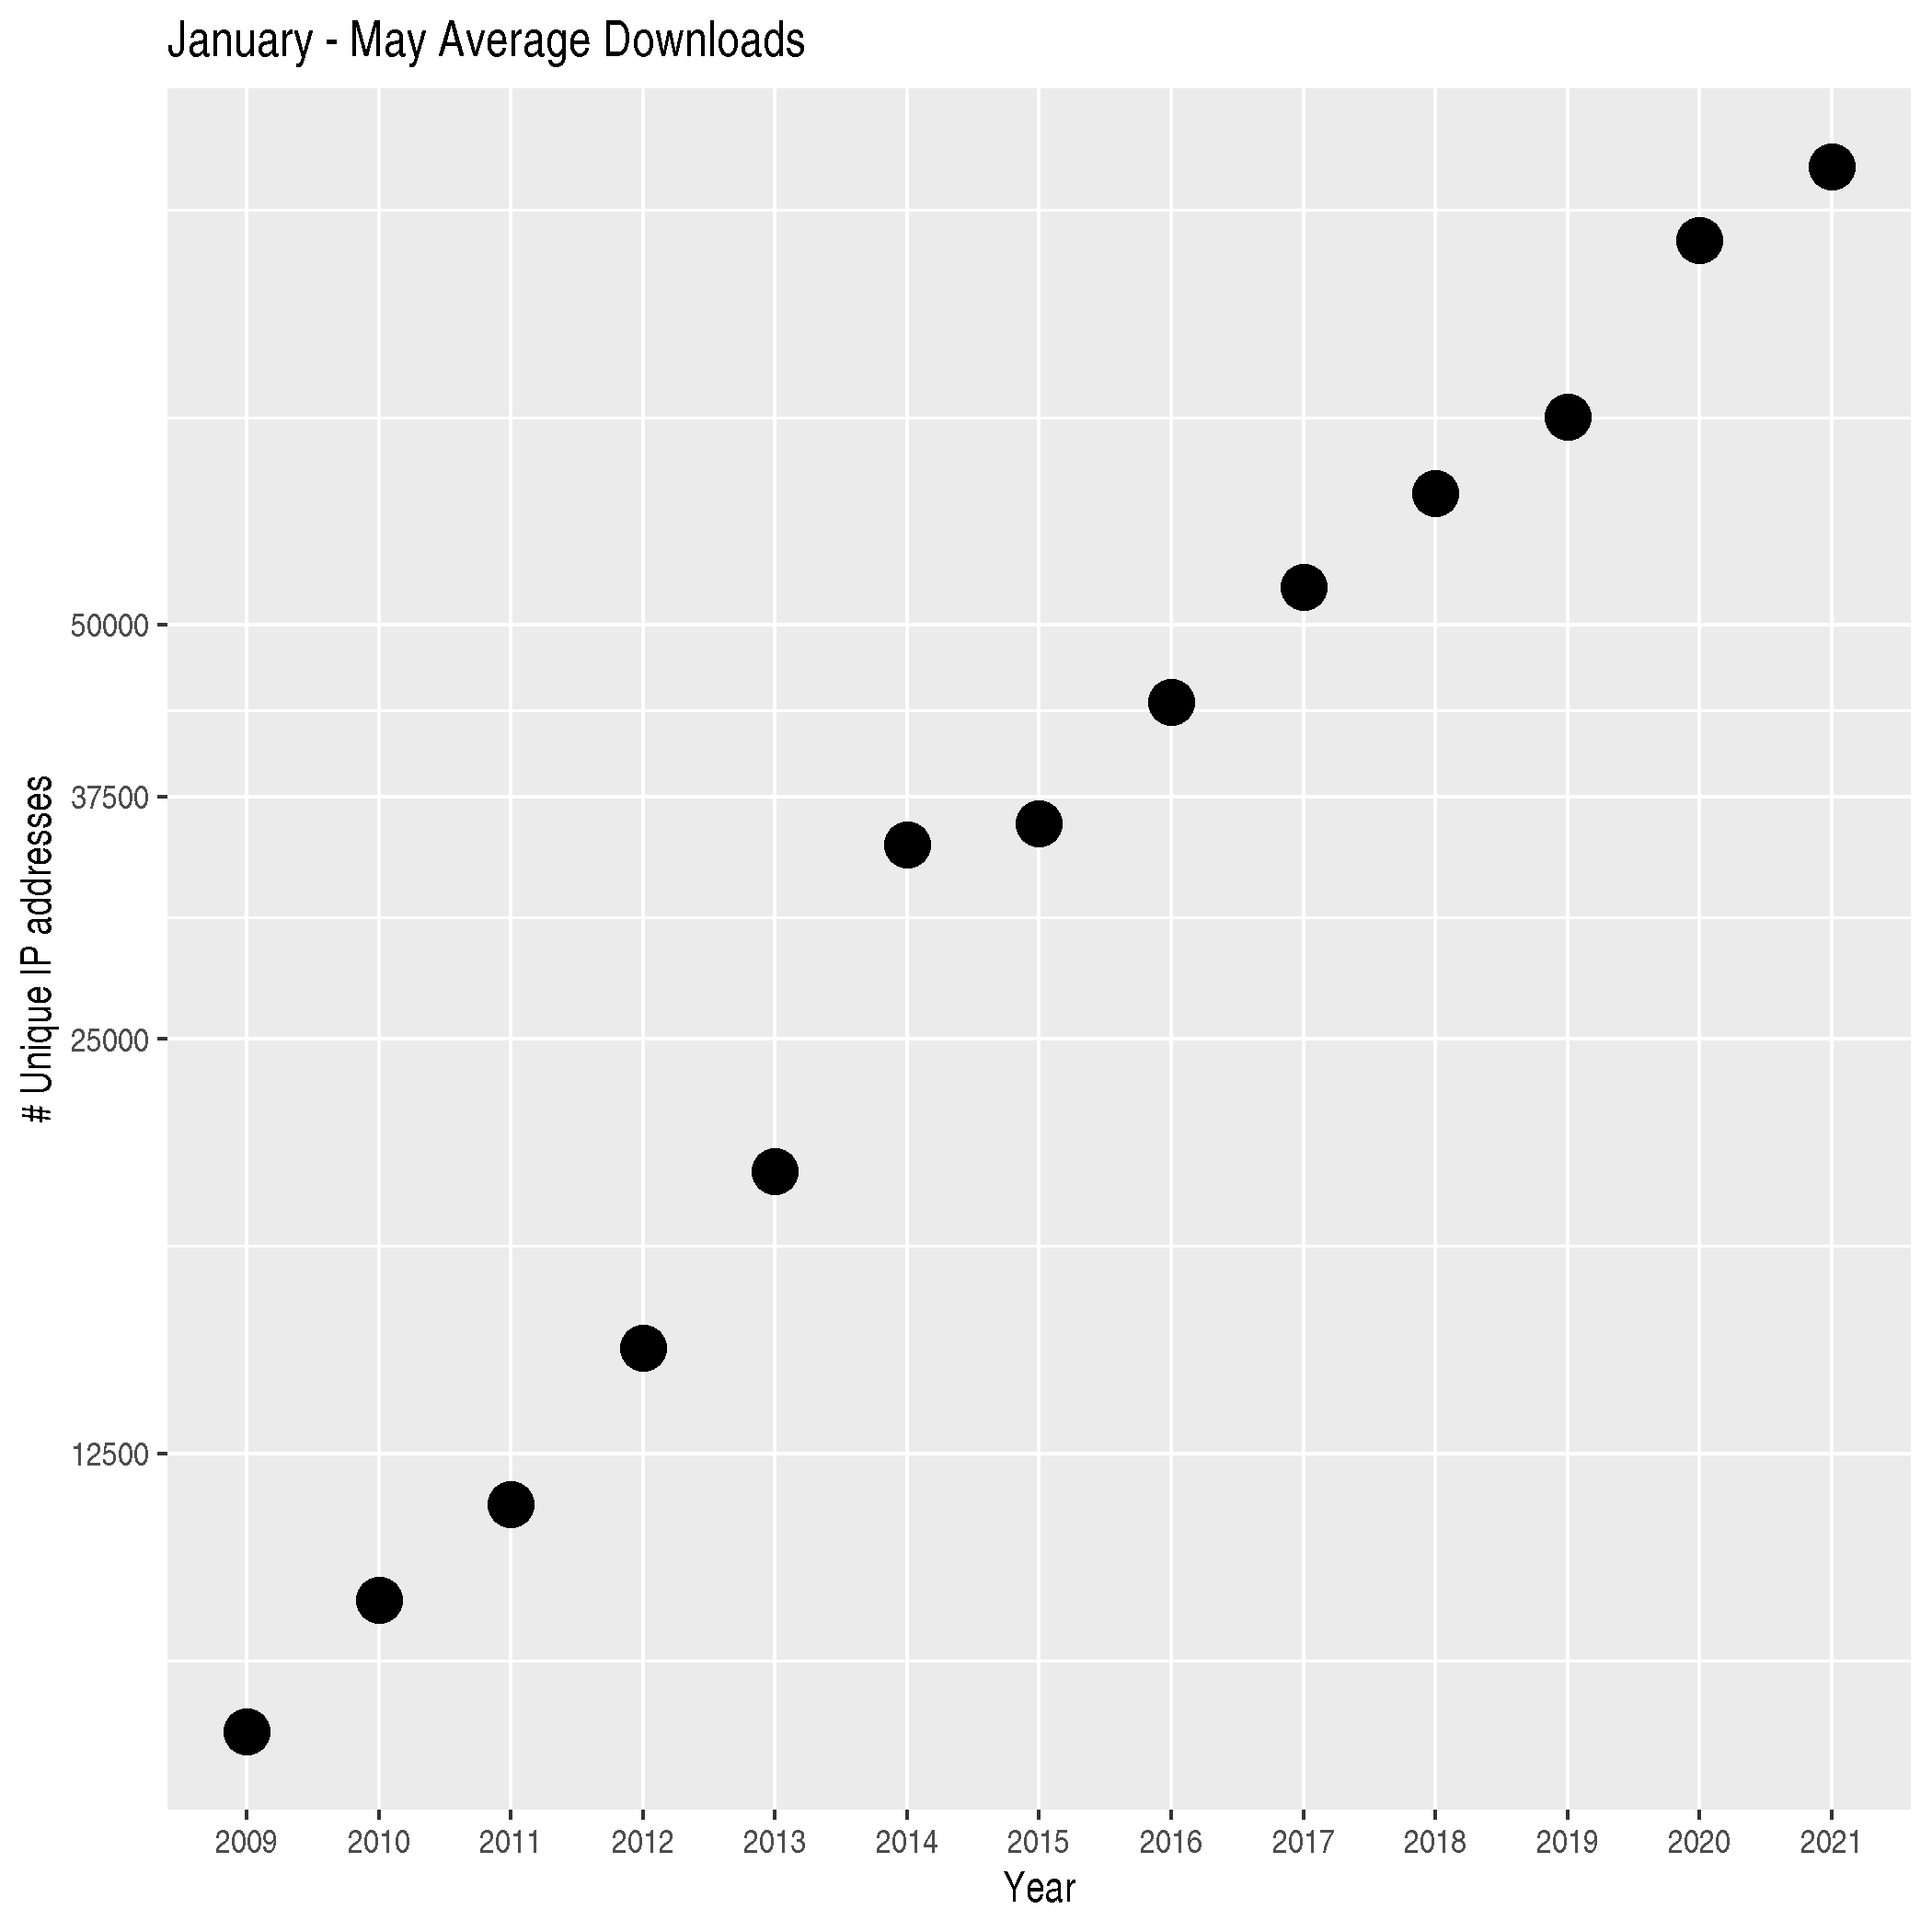
\includegraphics[width=.5\textwidth,height=!]{download-stats-2021}
    \caption{\Bioconductor{} package download statistics, average number
      of unique downloads, first six months of each year.}
    \label{fig:download-stats}
  \end{center}
\end{figure}


\subsection{Courses and Conferences}

Our annual conferences include:

\begin{itemize}
\item \href{https://bioc2021.bioconductor.org}{BioC2021} North American
  conference was held as a 3-day virtual conference from August 4-6; no in
  person components due to continued covid 2019 restrictions. Participation
  reached 809 attendees.    
\item \href{https://biocasia2021.bioconductor.org/}{BioCAsia2021}, held
  as a virtual conference from November 1-4, 2021. Talks were multilingual
  translating to Japanese, Mandarin, and English. There were estimated 430
  attendees.
\item In conjunction with the \href{https://twitter.com/RBioinformatica}{Mexican Bioinformatics Network} and
the \href{https://twitter.com/nnb_unam}{Nodo Nacional de Bioinformática CCG UNAM},
the Comunidad de Desarrolladores de Software en Bioinformática
held two week-long
\href{https://comunidadbioinfo.github.io/post/cdsb-2021-workshops/#.YOgqyhNuelY}{online workshops}
addressing development of
\href{https://comunidadbioinfo.github.io/cdsb2021_workflows/}{workflows with RStudio and shiny} and
\href{https://comunidadbioinfo.github.io/cdsb2021_scRNAseq/}{analysis of single-cell RNA-seq experiments},
August 9-13, 2021.

\item \href{https://eurobioc2022.bioconductor.org/}{European
  Bioconductor Meeting}, was postponed to March 16-18, 2022.
\item Bioconductor workshops were also held as \href{https://www.h3abionet.org/categories/event/workshop/introduction-to-hands-on-bioconductor-workshop}{virtual workshops} in conjunction
  with \href{https://h3africa.org/}{H3Africa}.
\end{itemize}


The \href{https://bioconductor.org/help/course-materials/}{course
  materials} section of the web site summarizes material from these
and some of the many other courses and conferences offered by
\Bioconductor and the \href{https://bioconductor.org/help/events/}{events
  calendar} list conferences, workshops, and other events that involve
\Bioconductor.



\subsection{Community Support}

The \Bioconductor{} \href{https://support.bioconductor.org}{support
  site} is used for help, announcements, and outreach worldwide. From January
01, 2021 to November 30, 2021, there are 2400 new users, 1901 `top-level` posts,
and 4933 comments (answers+comments). 

The support site was upgraded and standardized to be consistent with the
Biostars code base. Natay Aberra from Biostars has been instrumental in the
transition; Lori Kern from the core team is working with Natay to be able to
update and troubleshoot as necessary. 


Another form of communication for the Bioconductor community is the \Bioconductor{}
\href{https://community-bioc.slack.com}{community slack}. As of November 30,
2021, there are 1615 members of the community slack channel with 97 different channels.


We continue to provide the
\href{http://www.stat.math.ethz.ch/mailman/listinfo/bioc-devel}{bioc-devel},
mailing list forum for package contributors' questions and discussion
relating to the development of \Bioconductor{} packages. There are
1811 subscribers on this list. Table~\ref{tbl:av_posts} lists the number of
posts and number of unique authors per month as a monthly average since
2002. Recent increase in activity is likely due to (1) enforced requirement that
new package maintainers subscribe to the mailing list, and (b) using
the bioc-devel mailing list as a support forum for use of
git.bioconductor.org. 

\begin{table}
\begin{center}
\caption{Monthly average number of posts and number of unique authors
  for the \Bioconductor{} 'devel' mail list from January, 2005. 2021 does not
  include December information}
\label{tbl:av_posts}
\begin{tabular}{lcc|lcc|lcc}
  \\
       & Posts     & Authors   &      & Posts     & Authors   &      & Posts     & Authors\\
  Year & per month & per month & Year & per month & per month & Year & per month & per month\\
  \hline\noalign{\smallskip}
  2005 & 27        & 13        & 2011 & 52        & 24        & 2017 & 186 & 45 \\
  2006 & 39        & 19        & 2012 & 75        & 25        & 2018 & 160 & 48 \\
  2007 & 50        & 23        & 2013 & 97        & 34        & 2019 & 123 & 44 \\
  2008 & 27        & 18        & 2014 & 139       & 41        & 2020 & 134 & 47 \\
  2009 & 26        & 17        & 2015 & 142       & 43        & 2021 & 104 & 38 \\
  2010 & 30        & 18        & 2016 & 153       & 45\\
\end{tabular}
\end{center}
\end{table}



\subsection{Publication}

\Bioconductor{} has become a vital software platform for the worldwide
genomic research community, with more than 38,500 PubMedCentral
full-text citations for `Bioconductor'. Table~\ref{table:pubMed}
summarizes PubMed author / title / abstract or PubMedCentral full-text
citations since 2003.

\begin{table}
  \caption{PubMed title and abstract or (2012 and later) PubMedCentral full text searches for ``Bioconductor'' on
    publications from January, 2003 -- July, 2020.}
  \label{table:pubMed}
  \begin{center}
    \begin{tabular}{rc|rc|rc|rc|rc}
      Year &  N & Year &  N & Year &    N & Year  & N    & Year  & N\\\hline\noalign{\smallskip}
      2003 &  7 & 2007 & 44 & 2011 &   68 & 2015  & 3138 & 2019  & 6010 \\
      2004 & 13 & 2008 & 52 & 2012 & 1386 & 2016  & 3415 & 2020 & 7655 \\
      2005 & 19 & 2009 & 62 & 2013 & 2048 & 2017  & 3988 & 2021 & 9141 \\
      2006 & 30 & 2010 & 52 & 2014 & 2401 & 2018  & 4610 & \\
    \end{tabular}
  \end{center}
\end{table}

\href{https://bioconductor.org/help/publications/}{Featured and recent
  publications} citing \Bioconductor{} are available on the
\Bioconductor{} web site, and are updated daily. 

\section{New and Ongoing Accomplishments}

\subsection{Leadership structure \& community engagement}

The \href{https://bioconductor.org/about/technical-advisory-board/}{Technical Advisory Board} meets
monthly to discuss technical issues important to establishing and
maintaining project momentum. Over the past three years the structure
has been formalized with a governance document and procedures to
ensure influx of new participants through a public nomination process
followed by election to a three year term. 
Meeting minutes are publised at the site noted above.

The \href{https://bioconductor.org/about/community-advisory-board/}{Community Advisory Board} was established in 2020 to more
directly address the training and outreach mission of
\Bioconductor.  The Community Advisory Board has developed
\href{guidelines}{http://workinggroups.bioconductor.org/working-group-and-committee-guidelines.html}
for creating new working groups and committees to harness community energies.  Active working
groups work in the following areas:
\begin{itemize}
\item \href{https://github.com/Bioconductor/bioc_coc_multilingual}{Code of conduct}.
\item Conference planning.
\item \href{http://bioconductor.org/developers/new-developer-program/}{Developer training} (\href{https://www.youtube.com/watch?v=CcJgcDy2qEI&list=PLdl4u5ZRDMQQLMupAtEzm2y4gUIUm_1n6}{youtube playlist}).
\item \href{https://github.com/bioconductor/bioconductor-teaching}{Education} (including \href{https://github.com/carpentries-incubator/bioc-intro}{Carpentries incubator modules}).
\item Governance, which has included engagement with La Piana consulting, a national firm advising on 
strategies for non-profits.
\end{itemize}

\subsection{User Support}

\begin{description}
\item[\href{https://support.bioconductor.org}{Support site}] has
  established itself as an important resource. We have been engaged in
  an extended collaboration with Biostars author to harmonize our code
  base with upstream code, to enhance security, and to prepare for the
  release of an updated support forum.
\item[\href{https://bioconductor.org/help/workflows}{Workflows}]
  provide cross-package training material and integrate with the
  \href{http://f1000research.com/channels/bioconductor}{F1000
    \Bioconductor{} channel}. Workflows are now distributed as
  standard \R{} packages built regularly, distributed through
  CRAN-style repositories, and organized on the web site using the
  same approach as other package types.
\item[\href{https://community-bioc.slack.com}{Slack}] channels for the
  core team and \Bioconductor{} community are providing new avenues
  for communication. The community slack channel was an important
  catalyst in the HCA grantsmanship process, and in several
  significant collaborative software initiatives lead by community
  members.
\item[\href{https://bioconductor.org/help/course-materials}{Course
    Materials}] organize and make accessible recent course and
  training material.
\end{description}

\section{Core Tasks \& Capabilities}

\subsection{Core Tasks}

\begin{enumerate}

\item Package Building and Testing.  The \Bioconductor{} project
  provides access to its packages through repositories hosted at
  \texttt{bioconductor.org}.  One of the services provided to the
  \Bioconductor{} community is nightly automated build and check of
  all packages.  Maintaining the automated build and test suite and
  keeping the published package repositories updated requires a
  significant amount of time on the part of the Roswell
  \Bioconductor{} team.  As the project has grown, the organizational
  and computational resources required to sustain the package build
  system have also increased; see section~\ref{sec:pkg_building}.

\item Package dissemination via
  \href{https://bioconductor.org}{https://bioconductor.org} and
  underlying CRAN-style repository using Amazon CloudFront for global
  distribution.

\item Software development.

\item End-user support via
  \href{https://support.bioconductor.org}{https://support.bioconductor.org}
  and the bioc-community slack channel.

\item Developer support via the
  \href{https://stat.ethz.ch/mailman/listinfo/bioc-devel}{bioc-devel}
  mailing list.

\item New package submission.  The \Bioconductor{} project relies on
  technical review process of candidate packages to ensure they
  contain high-quality software.

\item Annotation data packages.  The \Bioconductor{} project
  synthesizes genomic and proteomic information available in public
  data repositories in order to annotate genomic sequences and probes
  of standard microarray chips.  These annotation data packages are
  made available to the community and allow \Bioconductor{} users to
  easily access meta data relating to their experimental platform.  We
  maintain automated tools to parse the available information.

\item Semi-annual releases, typically in March and October.

\end{enumerate}

\subsection{Hardware and Infrastructure}
\label{sec:pkg_building}

The \Bioconductor{} project provides packages for computing platforms
common in the informatic community.  We provide source packages
that can be installed on Linux and most UNIX-like variants, as well as
binary packages for Windows and macOS.  To ensure that packages are
consistently documented, easy to install, and functioning properly, we
run a nightly build during which we test all packages in the release
and development repositories.  

The build system currently consists of at least two Windows machines,
two Linux machines, and two macOS machines. The Windows, Linux, and
one macOS machines are physical servers located at Roswell Park, the
remaining macOS machine is rented via MacStatdium. The web site,
support site, AnnotationHub, and additional servers are hosted on
virtual machines, some of which are Amazon machine instances. The
build machines are recently updated, with adequate room for growth.

\subsection{Key Personnel}
\label{sec:key_personnel}

The \textbf{Core Development Team} 
develops software and other infrastructure
and ensures day-to-day operation of the project. Core team members in
the period covered by this report include Martin Morgan, Vincent Carey, Herv\'{e}
Pag\`{e}s, Marcel Ramos, Lori Shepherd, Nitesh Turaga,
and Kayla Interdonato. 

\section{Advisory Boards}

The \textbf{Technical Advisory Board} provides guidance through
monthly telephone conference calls.  Table \ref{tabtable}
lists members as of October 2022 (sic).

% latex table generated in R 4.2.1 by xtable 1.8-4 package
% Sun Oct 16 06:40:42 2022
\begin{table}[ht]
\label{tabtable}
\caption{Technical advisory board members serving as of Oct. 2022.}
\centering
\begin{tabular}{llll}
  \hline
 Name & Organization & City & Country \\ 
  \hline
 Vince Carey & Harvard Medical School & Boston & US \\ 
 Levi Waldron & CUNY School of Public Health & New York & US \\ 
 Charlotte Soneson & FMI & Basel & CH \\ 
 Aedin Culhane & U Limerick & Limerick & IE \\ 
 Sean Davis & University of Colorado Anschutz Medical Campus & Aurora & US \\ 
 Laurent Gatto & Université Catholique de Louvain & Louvain-la-Neuve & BE \\ 
 Robert Gentleman & Harvard Medical School & Boston & US \\ 
 Shila Ghazanfar & Cancer Research UK Cambridge Institute & Cambridge & GB \\ 
 Kasper Daniel Hansen & Johns Hopkins University & Baltimore & US \\ 
 Stephanie Hicks & Johns Hopkins Bloomberg School of Public Health & Baltimore & US \\ 
 Wolfgang Huber & EMBL & Heidelberg & DE \\ 
 Rafael Irizarry & Dana-Farber Cancer Institute & Boston &  US \\ 
 Lori Shepherd & Roswell Park Cancer Institute & Buffalo & US \\ 
 Michael Love & University of North Carolina at Chapel Hill & Chapel Hill & US \\ 
 Davide Risso & University of Padua & Padova & IT \\ 
   \hline
\end{tabular}
\end{table}


The \textbf{Community Advisory Board} supports the
\Bioconductor{} mission by empowering user and developer communities
by coordinating training and outreach activities, and enabling
productive and respectful participation by Bioconductor users and
developers at all levels of experience.  See \ref{cabtable} for
member information.

% latex table generated in R 4.2.1 by xtable 1.8-4 package
% Sun Oct 16 05:58:14 2022
\begin{table}[ht]
\centering
\label{cabtable}
\caption{Community advisory board members serving as of Oct. 2022.}
\begin{tabular}{llll}
  \hline
  Name & Organization & City & Country \\ 
  \hline
 Yagoub A. I. Adam & Covenant University & Ota & NG \\ 
   Benilton Carvalho & Universidade Estadual de Campinas & Campinas & BR \\ 
   Daniela Cassol & University of California Riverside & Riverside & US \\ 
   Leonardo Collado-Torres & Lieber Institute for Brain Development & Baltimore & US \\ 
   Aedin Culhane & Dana Farber Cancer Institute & Boston & US \\ 
   Xueyi Dong & Walter and Eliza Hall Institute of Medical Research & Melbourne & AU \\ 
   Susan Holmes & Stanford University & Stanford & US \\ 
   Leo Lahti & University of Turku & Turku & FI \\ 
   Estefania Mancini & Centre for Genomic Regulation & Barcelona & ES \\ 
   Kozo Nishida & RIKEN & Suita & JP \\ 
   Nicole Ortogero & Nanostring, Inc. & Seattle & US \\ 
   Johannes Rainer & Eurac Research & Bolzano & IT \\ 
   Janani Ravi & University of Colorado Anschutz Medical Campus & Aurora & US \\ 
   Matt Ritchie & Walter and Eliza Hall Institute of Medical Research & Melbourne & AU \\ 
   Kevin Rue-Albrecht & University of Oxford & Oxford & GB \\ 
   Lori Shepherd & Roswell Park Cancer Institute & Buffalo & US \\ 
   Mike Smith & EMBL & Heidelberg & DE \\ 
   Hedia Tnani & CNAG & Barcelona & ES \\ 
   \hline
\end{tabular}
\end{table}


The \textbf{Scientific Advisory Board} provides oversight through
yearly meetings.  No meeting was held in 2021.  Board
membership as of October 2022 is listed in Table \ref{sabtable}.

\begin{table}[ht]
\centering
\caption{Scientific Advisory Board members.}
\label{sabtable}
\begin{tabular}{rllll}
  \hline
 Name & Organization & City & Country \\ 
  \hline
 Robert Gentleman & Harvard Medical School & Boston & US \\ 
 Rafael Irizarry & Dana-Farber Cancer Institute & Boston & US \\ 
 Vincent Carey & Harvard Medical School & Boston & US \\ 
 Chris Wellington & NHGRI & Bethesda & US \\ 
 Wolfgang Huber & EMBL  & Heidelberg & DE \\ 
 Martin Morgan & Roswell Park Comprehensive Cancer Center & Buffalo & US \\ 
 Benjamin Neale & Broad Institute & Cambridge & US \\ 
 Michael Schatz & Johns Hopkins University & Baltimore & US \\ 
 Aviv Regev & Genentech, Inc. & San Francisco & US \\ 
 Sandrine Dudoit & UC Berkeley & Berkeley & US \\ 
 John Marioni & EMBL-EBI & Cambridge & GB \\ 
 Daniela M Witten & U Washington & Seattle & US \\ 
 Barbara Engelhardt & Stanford University & Stanford & US \\ 
 Susan Holmes & Stanford University & Stanford & US \\ 
 Benilton Carvalho & Universidade Estadual de Campinas & Campinas & BR \\ 
 Jay Shendure & University of Washington & Seattle & US \\ 
   \hline
\end{tabular}
\end{table}


\end{document}
